In this section, I explain the data analysis, cleaning, transformation, feature engineering, and models.

\section{Cleaning pointing scan data}
\subsection{Cleaning rules}
The pointing scan data is noisy, and contains a lot of outliers. In order to make the data more suitable for machine learning, we need to clean the data.
Below is a list of some criteria we use to filter out scans.
\begin{itemize}
    \item Scans using the HOLO transmitter. These scans are aiming at a radio tower, and is therefore not realistic data to train the ML model with.
    \item Scans using ZEUS2. These are highly experimental pointing scans and unreliable.
    \item Scans using CHAMP690, as there are very few scans using this instrument.
    \item Scans in January and February. There are not many scans in this time period, and the few we have involve a lot of testing.
    \item Scans that are tracking tests.
\end{itemize}   
\textcolor{red}{Find the proportion of scans that are removed from the above list.}
After this filtering, there are x out of 8862 scans left.
        
\subsection{Pointing scan classifier}
\subsubsection{Method}
In addition to the cleaning rules, we have to remove the ouright bad pointing scans (like \ref{subfig:bad_continuous} \ref{subfig:bad_line}, \ref{subfig:bad_line}).
This is done by training a classifier predict whether a scan is good or bad.
We used an XGBoost classifier with 13 features as inputs, all of which are present in the pointing scan figures (\ref{fig:line_pointings} and \ref{fig:continueous_pointings}).
The first 12 features are the amplitudes, FWHMs and pointing offsets, along with the uncertainties of these values.
The last feature is the beamsize of the telescope for the given observing frequency.\\

We had to label a training set by manually looking at pointing scans.
The size of the training set was $369$ with $270$ good and $99$ bad scans.
We did a hyperparameter search for the max depth between $1$ and $5$, number of estimators between $1$ and $80$, 
and used the \textit{scale\_pos\_weight} to consider the unbalanced classes. The value for this parameter is the ratio of negative to positive classes.
$80\%$ of the data was used for training, and the rest for testing, which corresponds to $295$ and $74$ samples for training and testing respectively.


\begin{itemize}
    \item What hyperparameters were tuned, and what are the values.
    \item Show why it is hard to clean by only noise
    \item labeling trainig set manually, size and proportion of pos neg
    \item can choose how strict we want to be on the cleanliness
    \item precicion recall curve or mAP curve?onda
\end{itemize}

\subsubsection{Results}
The XGBoost classifier performed well a $97\%$ overall accuracy on the test set.
Figure \ref{fig:pointing_scan_clf} shows the precicion-recall curve on the left and the average precision curve on the right.
From the precision-recall curve it is clear that we can achieve a close to $100\%$ precision while still having a high recall.
This is ideal, as we want the training data for the pointing model to be as clean as possible.
We can select a large threshold, such that very few bad scans end up in the training data.
The average precicion curve shows an optimal threshold for maximizing the precision, which is about $80\%$.

\begin{figure}[H]
    \centering
    \begin{subfigure}[t]{0.49\textwidth}
        \centering
        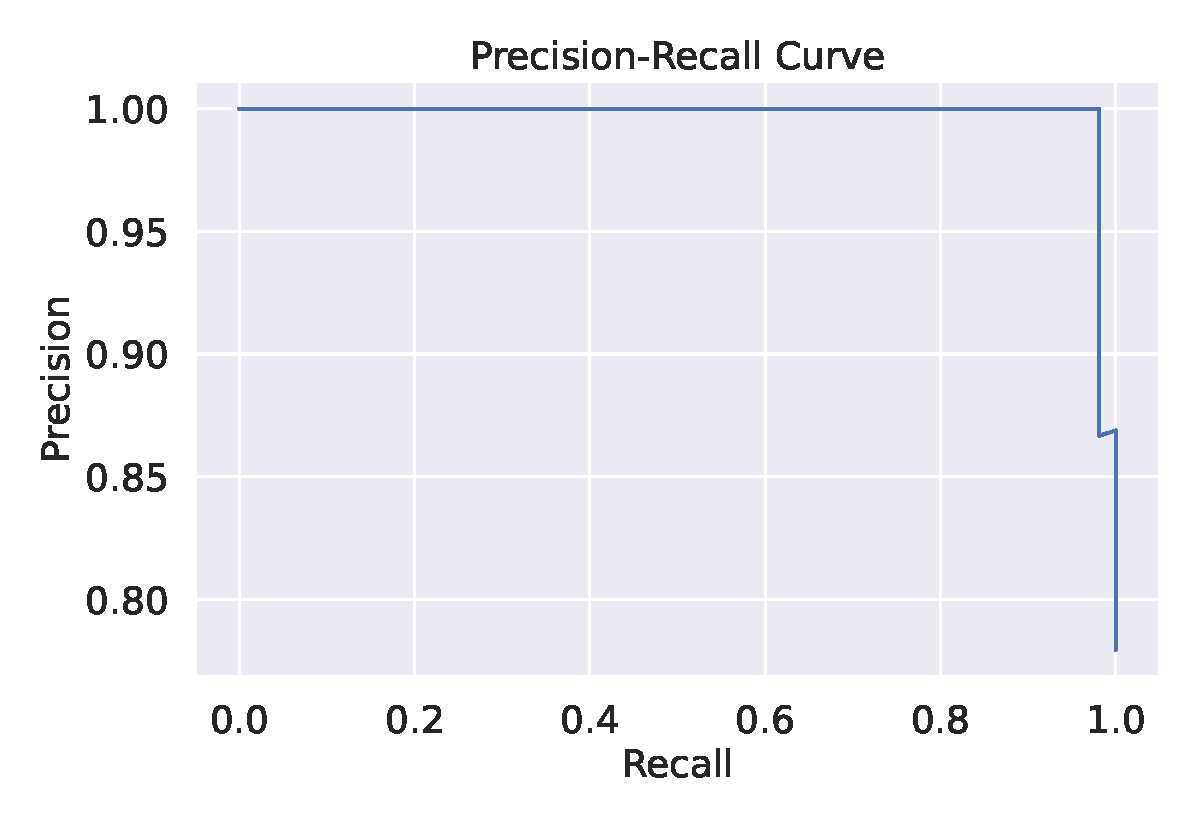
\includegraphics[width=1\textwidth]{Clf/precision_recall_curve_both.pdf}
        \caption{Precision-recall curve on test set.}
        \label{subfig:pr_curve}
    \end{subfigure}
    \begin{subfigure}[t]{0.49\textwidth}
       \centering
       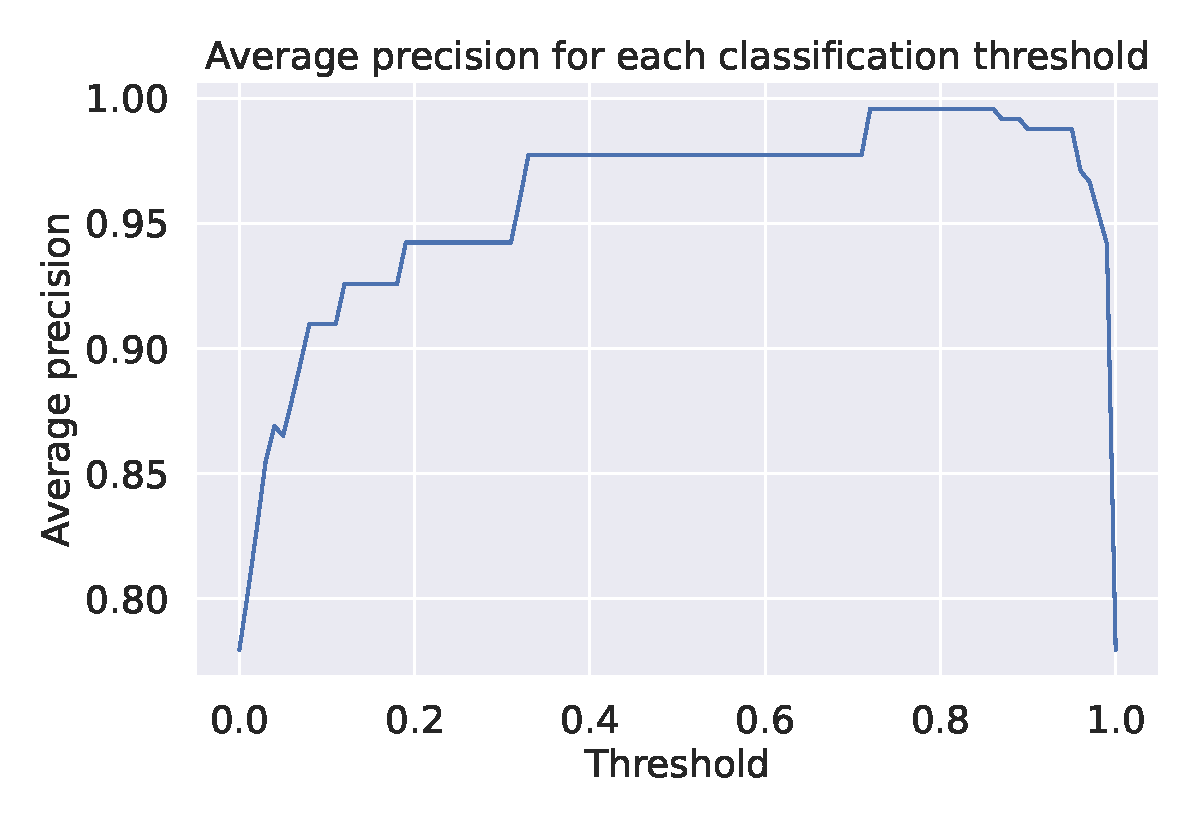
\includegraphics[width=1\textwidth]{Clf/mAP_curve_both.pdf}
       \caption{Average precision for different classification threshold.}
       \label{subfig:map_curve}
    \end{subfigure}
     \caption{Precision-recall and average precision curve for the XGBoost classifier when classifying good and bad pointing scans in the test set.}
     \label{fig:pointing_scan_clf}
\end{figure}

% \\~\\
% \begin{subfigure}[t]{0.49\textwidth}
%     \centering
%     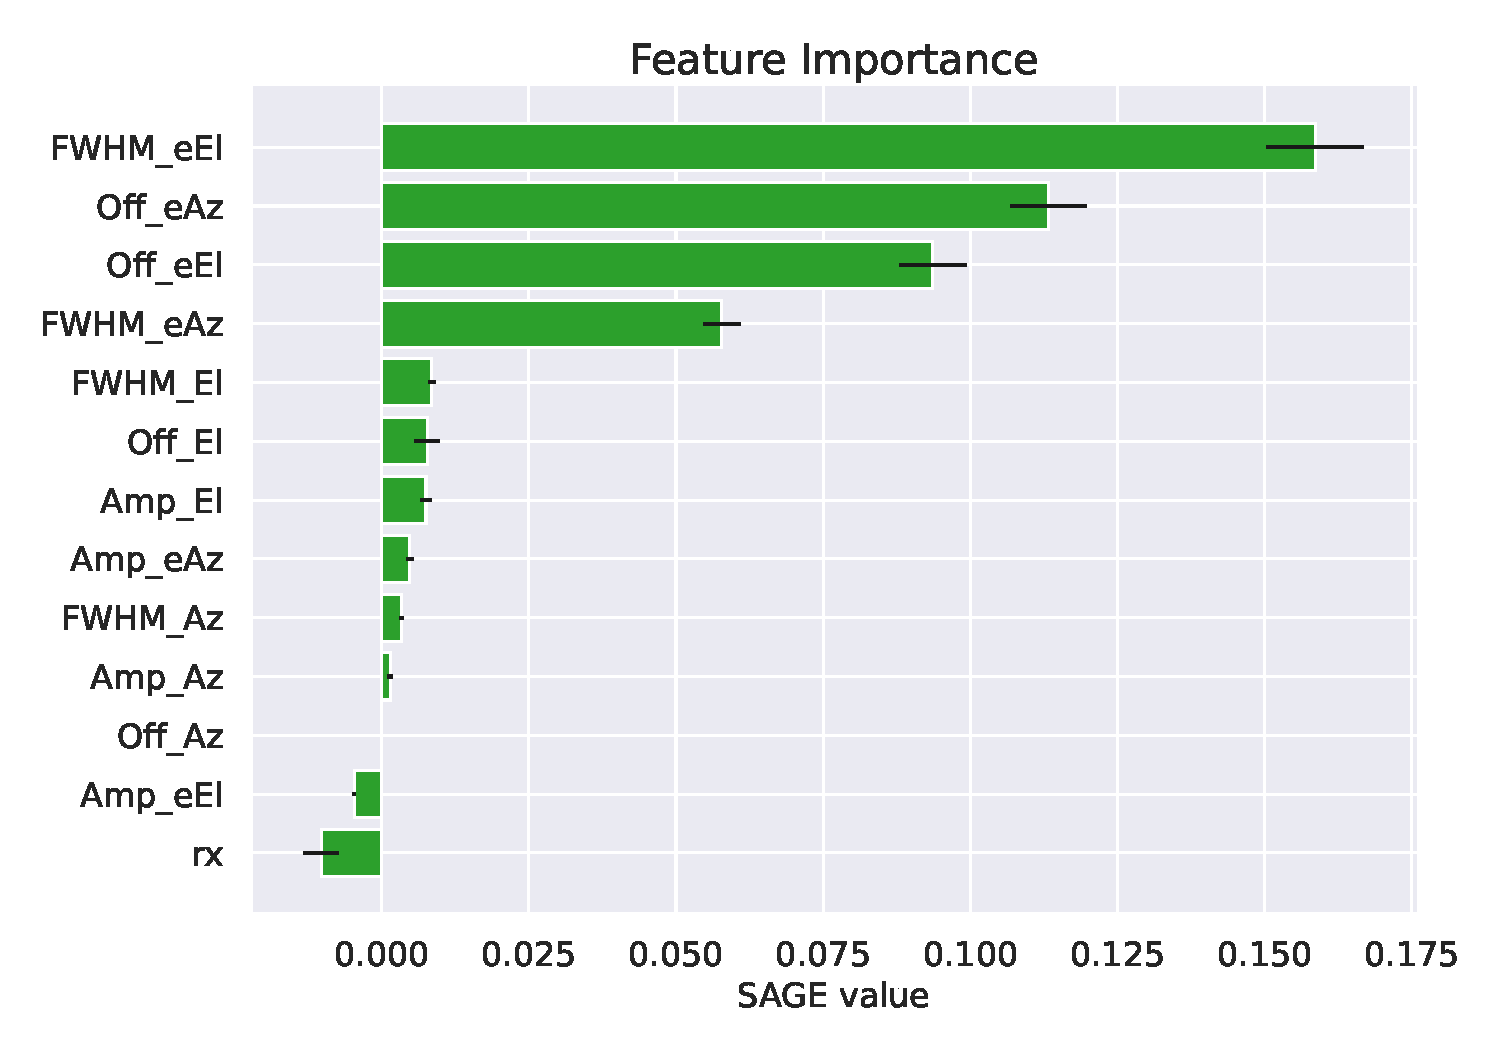
\includegraphics[width=1\textwidth]{Clf/Sage_xgb_clf_rx.pdf}
%     \caption{Average precision for different classification threshold.}
%     \label{subfig:xgb_clf_sage}
% \end{subfigure}
% \begin{figure}[H]
%     \centering
%     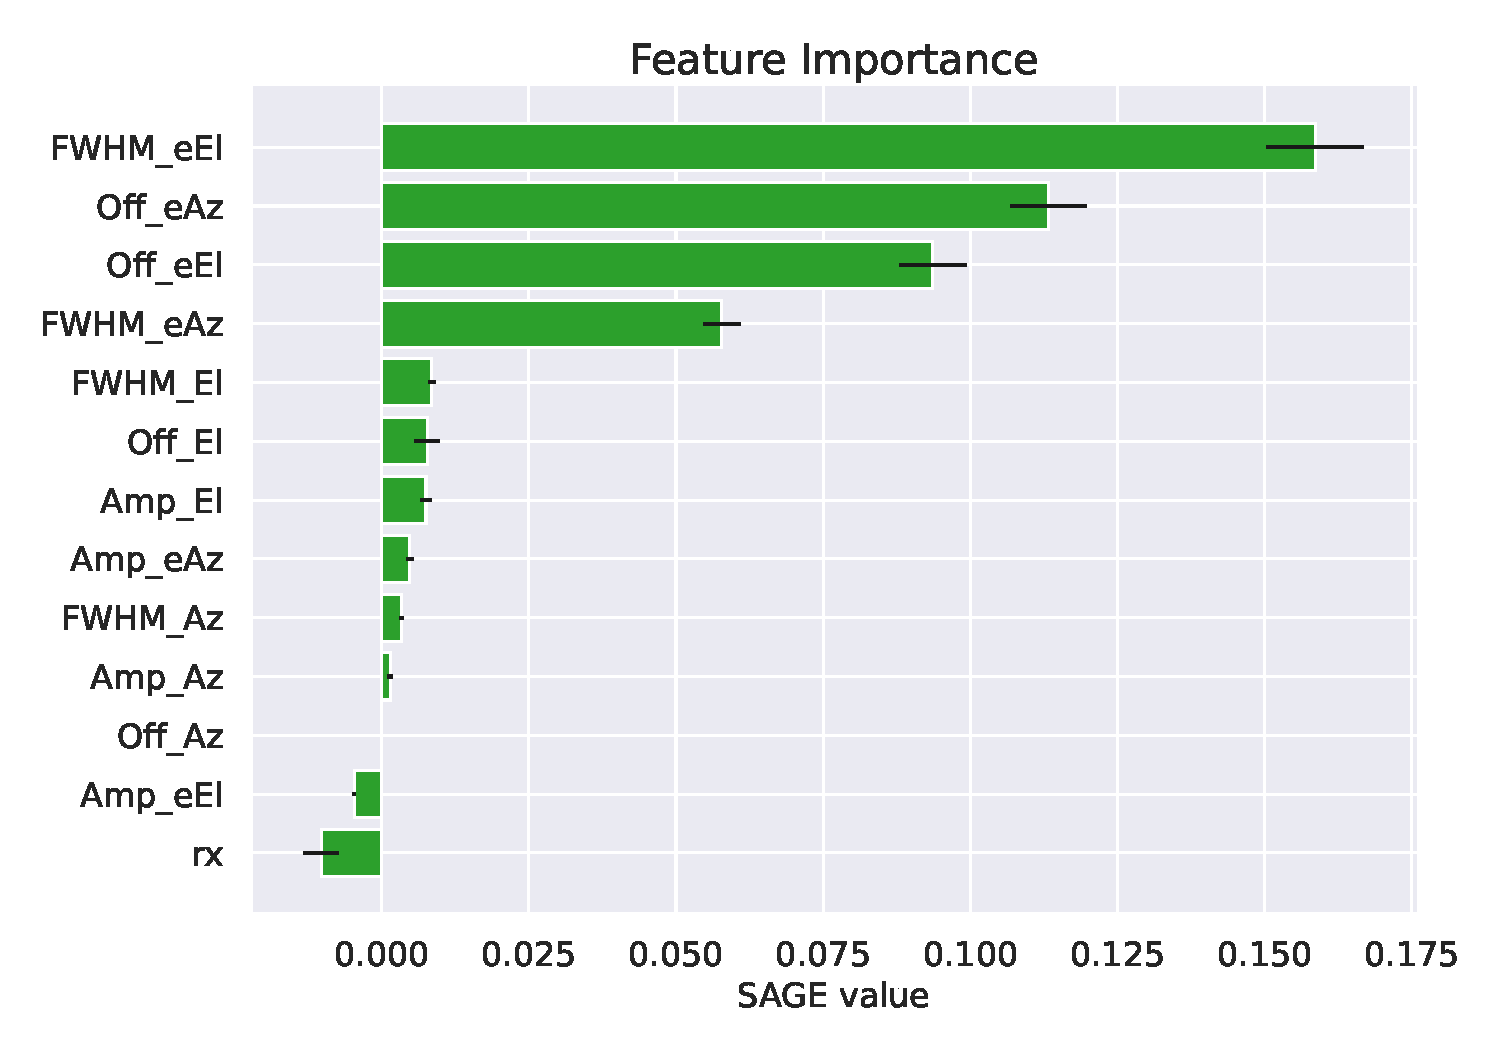
\includegraphics[width=0.98\textwidth]{Clf/Sage_xgb_clf_rx.pdf}
%     \caption{SAGE values for the XGB classifier.}
%     \label{fig:xgb_clf_sage}
% \end{figure}

\section{Scan duration analysis}
As mentioned in the database section, the timestamps of the scans is not the accurate start time of a scan.
The tiltmeter dump files with the flag indicating whether the telescope is idle, preparing to observe, or observing,
is the only data we have on when the telescope is actually performing a pointing scan.
Therefore, we need to combine the timestamp of the pointing scan with the flag in the dump files to analyse the duration of scans.

\subsection{Method}
First, we convert the different scan flags to numbers.
\textit{IDLE} and \textit{PREPARING} is the set $0$, and \textit{OBSERVING} is set to $1$.
Then we can subtract the previous rows from all rows, which will result in a value of $1$ when the scan starts, and $-1$ when it ends.
Table \ref{tab:scan_flag_difference} shows an example of the resulting table.


\begin{table}[H]
    \centering
    \begin{tabular}{cccc}
        \toprule
        Time & Flag & Flag Integer & $\Delta$ \\
        \midrule
        11:21:21 & IDLE & $0$ & $0$ \\
        11:21:22 & PREPARING & $0$ & $0$ \\
        11:21:23 & OBSERVING & $1$ & $1$ \\
        11:21:24 & OBSERVING & $1$ & $0$ \\
        11:21:25 & OBSERVING & $1$ & $0$ \\
        11:21:26 & IDLE & $0$ & $-1$ \\
        \bottomrule
    \end{tabular}
    \caption{This table shows the tiltmeter dump file containing the telescope state flag,
            and how we find the start ($\Delta = 1$) and end ($\Delta = -1$) of a scan.}
    \label{tab:scan_flag_difference}
\end{table}

By analyzing these tables for all the scans we had tiltmeter dumps for,
we see that the first \textit{OBSERVING} flag present after a scan is about $53$ \textcolor{red}{Add accurate mean and standard deviation} seconds after the scan timestamp for the vast majority of the scans.
This is shown in the right plot in figure \ref{fig:scan_times_box}, which strongly indicates that this is the starting point of a pointing scan.
In the same plot, we also see that this is fairly constant for the different instruments.
The right plot of figure \ref{fig:scan_times_date} show the time difference in seconds between the first observing flag after a scan timestamp throughout the year.
From the plot, we may conclude that this stays constant over time.\\

Now that we have found the start of a pointing scan, we look at the durations of the scans. 
The left plots in figure \ref{fig:scan_times_date} and \ref{fig:scan_times_box} show the duration of the pointing scans for different instruments.
From this figure, it is clear that the duration of a pointing scan varies a lot.
This is problematic because of the fact that we only have these tiltmeter dump files for $2862/8381\approx 34\%$ of the pointing scans.


\begin{figure}[H]
    \centering
    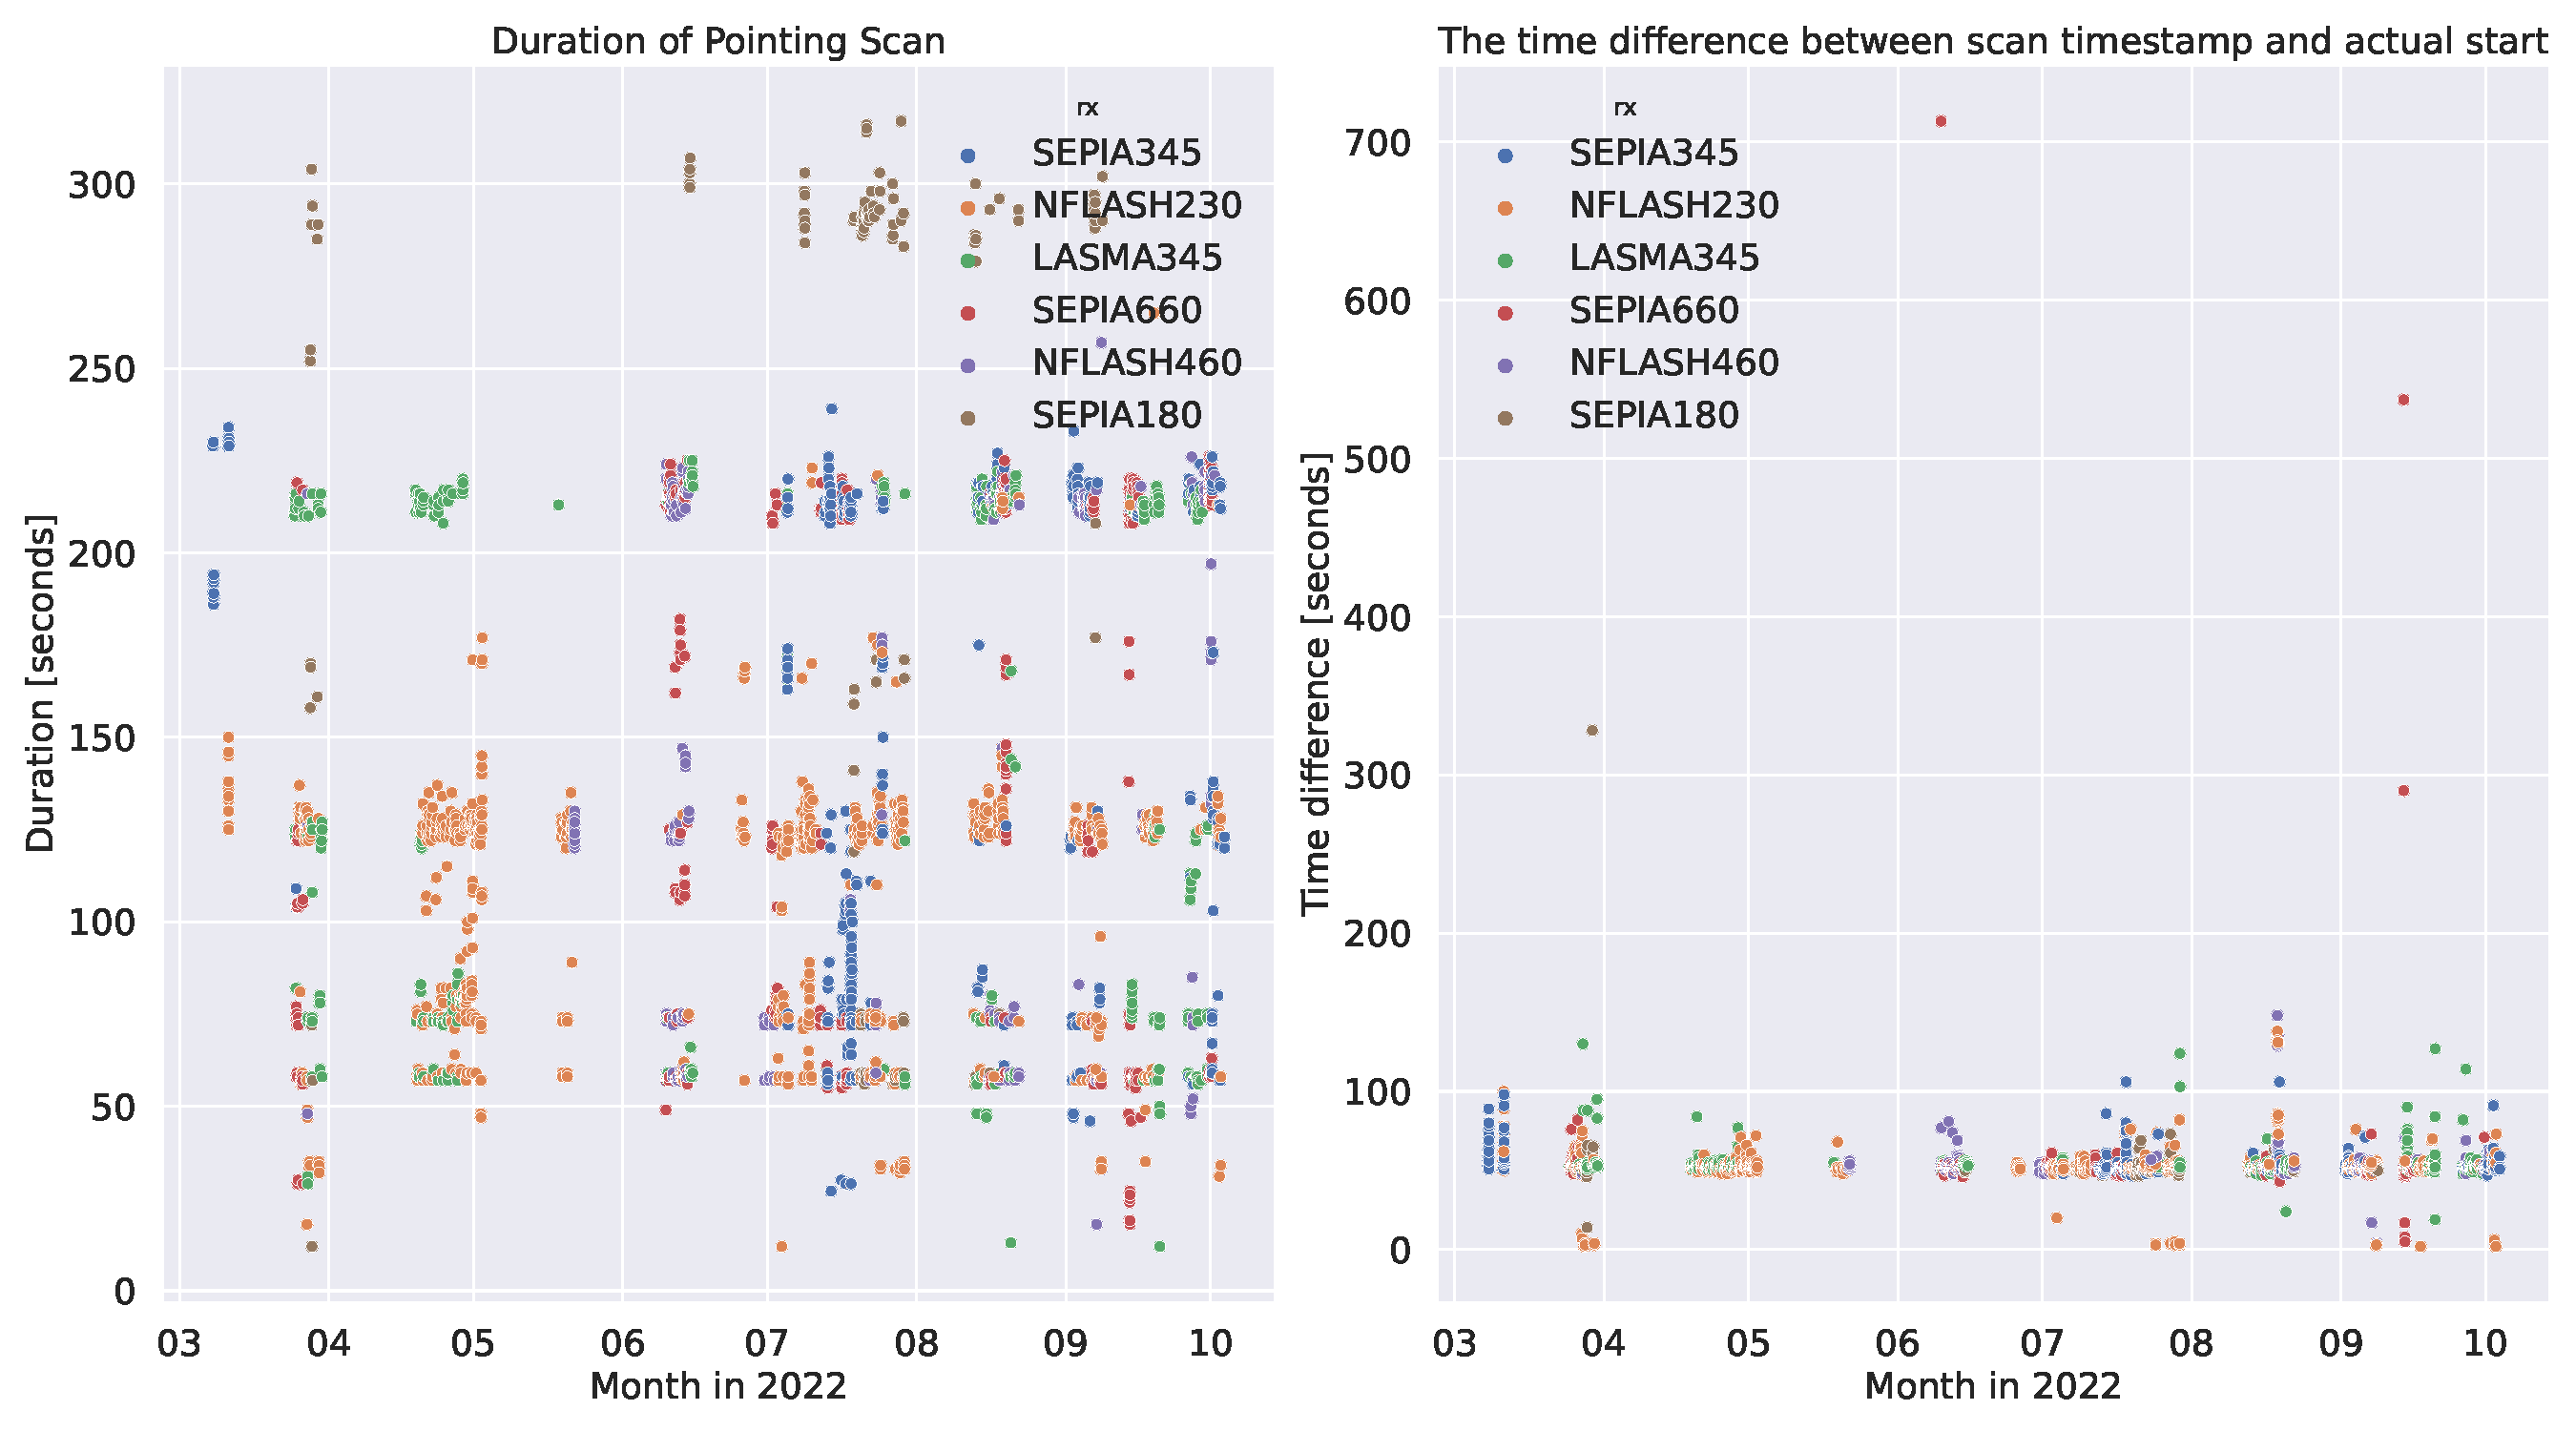
\includegraphics[width=1.1\textwidth]{Tiltmeter plots/scan_duration_distribution_date.pdf}
    \caption{Scatter plot of the duration of scans, and the time difference between the timestamp of a scan and the actual start of it.}
    \label{fig:scan_times_date}
\end{figure}

\begin{figure}[H]
    \centering
    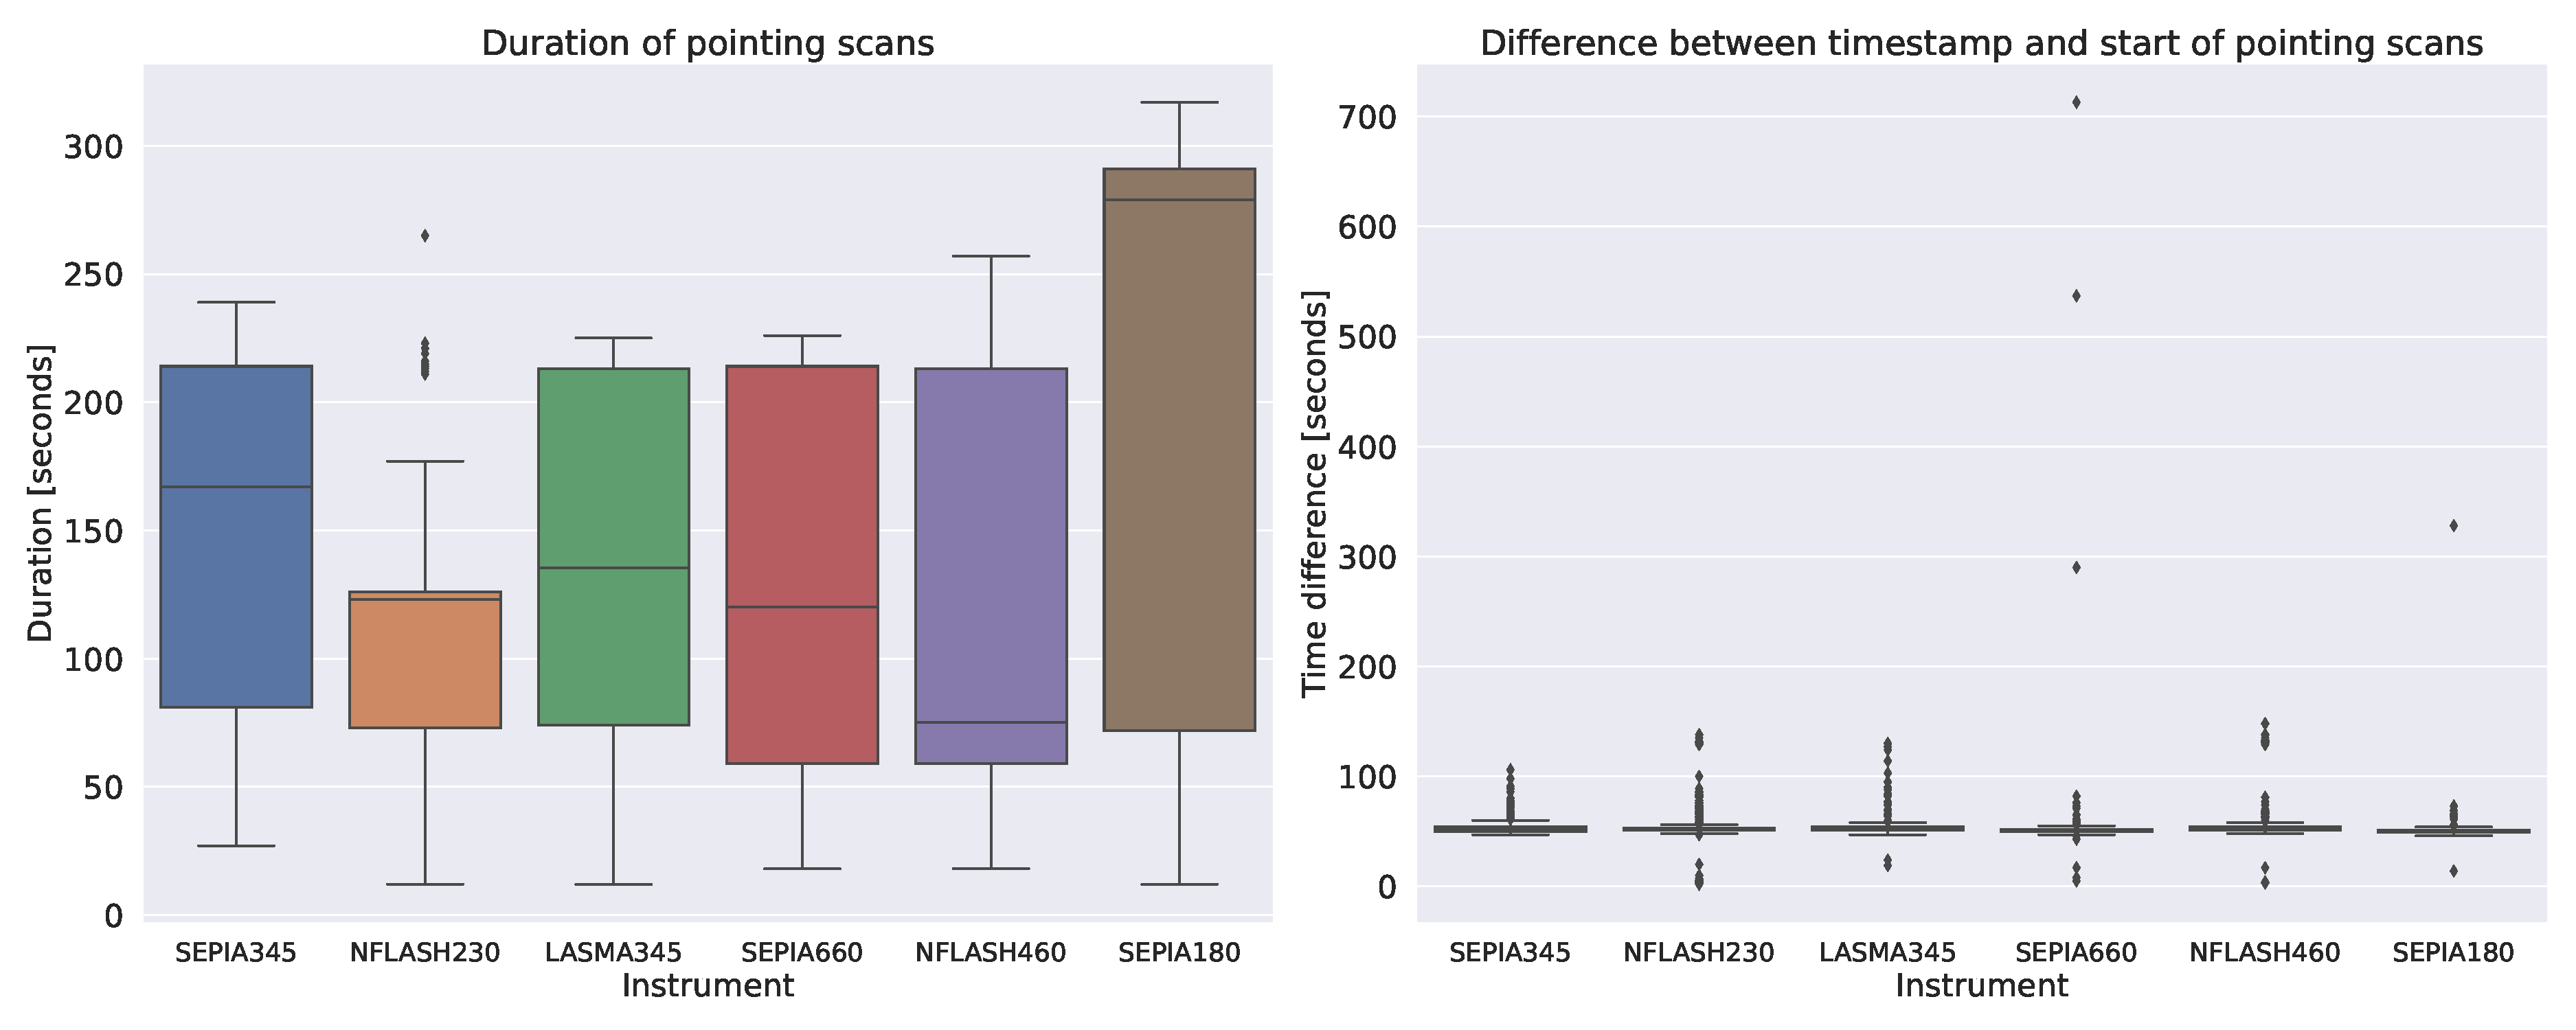
\includegraphics[width=1.1\textwidth]{Tiltmeter plots/scan_duration_distribution_rx.pdf}
    \caption{Box plot of the duration of scans, and the time difference between the timestamp of a scan and the actual start of it.}
    \label{fig:scan_times_box}
\end{figure}


\subsection{Algorithm}
Following is the algorithm used to obtain the start and end of pointing scans using the scan timestamp and the observing flag from tiltmeter dumps.

\begin{algorithm}[H]
    \caption{Find start and end of pointing scan}
    \label{alg:scan_times}
    \begin{algorithmic}
        \Require{\\
        \begin{itemize}
            \item Pointing scan timestamps $D=\{D_1,\dots,D_n\}$
            \item Timestamps $T=\{T_1,\dots,T_m\}$ and scan flag $F=\{F_1,\dots,F_m\}$
        \end{itemize}}
        \Ensure{Start and end of pointing scans $S=\{S_i,\dots,S_n\}$ and $E=\{E_i,\dots,E_n\}$}
        \For{$i=1,\dots,m$}
            \If {$F_i=OBSERVING$}
                \State {$F_i = 1$}
            \Else
                \State {$F_i = 0$}
            \EndIf
        \EndFor
        \\
        \For{$i=1,\dots,n$}
            \State {$\hat{T} = \{T_j, \text{  if  } T_j > D_i\}_j^m$}
            \State {$\hat{F} = \{F_j, \text{  if  } T_j > D_i\}_j^m$}
            \ForAll {$t_i,f_i \text{ in } \hat{T},\hat{F}$}
                \State {$\Delta = f_i-f_{i-1}$}
                \If {$\Delta = 1$}
                    \State {$S_i = t_i$}
                \EndIf
                \If {$\Delta = -1$}
                    \State {$E_i = t_i$}
                    \State {Continue}
                \EndIf
            \EndFor
        \EndFor
    \end{algorithmic}
\end{algorithm} 


\section{Feature Engineering}
\subsection{Different calculations}
There are two main types of features engineered for this project.
Features that represent the system during a pointing scan, and features that represent the changes since the last correction. 
The idea behind this is simple. The correction used during a pointing scan represent the ideal correction for the system during the previous pointing scan
As there are a lot of factors and complex relationships, and we don't have large amounts of training data, it might be easier for the model to learn 
how these changes affect the pointing rather than learning all the relationships.

\paragraph{Median values}
The median value of variables during a pointing scan is the most used feature.
Table \textcolor{red}{ref table with lsit of variables with median value} shows the list of variables for which we use the median values during a pointing scan.
\paragraph{Sum of all change}
To capture systematic error in pointing due to the telecope moving back and forth in azimuth and elevation,
we sum over the positive and negative change in these variables.

Given the time of the last pointing correction $t_1$ and the start of a pointing scan $t_2$, the sum over the positive changes in a variable $x_i$ is given by
\begin{equation}\label{eq:positive_int}
    \sum_{i=t_1+1}^{t_2} \max(0, x_i-x_{i-1})
\end{equation}

Similarly, the sum over negative changes in a variable is
\begin{equation}\label{eq:negative_int}
    \sum_{i=t_1+1}^{t_2} \min(0, x_i-x_{i-1})
\end{equation}

These features are made for azimuth and elevation.

\paragraph{Change since last correction}
This feature is self explanatory, and is just the change in a variable since the poining was corrected.
\begin{equation}
    \Delta x = x_{t_2} - x_{t_1}
\end{equation}

In order to make this feature more robust against noisy data,
we instead look at the change in the median for a time interval around the last corection $t_1$ and the start of a pointing scan $t_2$

\begin{equation}
    \Delta x = \textit{median}(x_{t_2}, x_{t_2 - 1}, \dots, x_{t_2- p}) - \textit{median}(x_{t_1}, x_{t_1 + 1}, \dots, x_{t_1 + p}),
\end{equation}
where $p$ is the number of data points needed to cover a period of $P$ minutes, given by $p = P \cdot frequency$. The unit of frequency is datapoints per minute, found in table \textcolor{red}{fix data freq ref}.

\paragraph{Max change in time interval}
In case the speed of the temperature change affects the deformation of the telescope's structure, we find the maximum temperature change in a given time interval since the last pointing correction.

\begin{equation}
    \max (x_{t_1+p} - x_{t_1}, x_{t_1+p} - x_{t_1}, \dots, x_{t_2} - x_{t_2-p}),
\end{equation}


\paragraph{Position of the sun}
Observers at the telescope report that the sun is affecting the pointing.
It is most drastically affected when the sun sets or rises, likely due to rapid change in temperature which leads to deformation in the telescope structure.
It is also thought that the position of the sun could play a role, and perhaps be modelled too.
For instance if the sun is shining on the left side of the telescope, it will affect the pointing differently than if it was on the right side.
Obtaining the position of the sun for the location of the telescope is done using the python module PyEphem \cite{ephem}.

Using the azimuth angle of the sun and the telescope, we can calculate the position of the sun with respect to the pointing with
\begin{equation}\label{eq:sun_az_diff}
    \Delta \textit{Az}_\odot = \textit{Az}_{\textit{t}} - \textit{Az}_\odot
\end{equation}
This will result in values outside the $[-180^\circ,180^\circ]$. An exampe of this is if $Az_\odot=179^\circ$ and $Az_t = -179^\circ$.
The calculation in equation \eqref{eq:sun_az_diff} yield $-179^\circ-179^\circ=-358^\circ$,
which corresponds to the sun being $358^\circ$ to the right of the telescope, while it ideally should be $2^\circ$ to the left.
Therefore, we adjust the values accordingly
%Write equations where \Delta Az_\odot above 180 is -= 360 and under 180 is += 360
\begin{align}
    \Delta Az_\odot = Az_\odot +360^\circ, \; \text{for} \; \Delta Az_\odot < 180^\circ\\
    \Delta Az_\odot = Az_\odot -360^\circ, \; \text{for} \; \Delta Az_\odot > 180^\circ
\end{align}

Here, the interval of the difference in azimuth is fixed to the interval $(-180^\circ,180^\circ)$,
where $0^\circ$ means the telescope is pointing towards the sun in azimuth direction.
$\Delta \textit{Az}_\odot = 90^\circ$ corresponds to the sun being directly to the left of the pointing direction. \\

Another measure tested is the total angle between the pointing and the position of the sun. This is calculated using the following formula
\begin{equation}
    \theta = \cos \textit{Az}_t \cdot \cos \textit{El}_t\cdot \cos \textit{Az}_\odot \cdot \cos \textit{El}_\odot + \sin \textit{Az}_t \cdot \cos \textit{El}_t\cdot \sin \textit{Az}_\odot \cdot \cos \textit{El}_\odot + \sin \textit{El}_t \cdot \sin \textit{El}_\odot
\end{equation}

\subsection{List of features}
\textcolor{red}{add list of all features for different calculations here}

\section{Transformation of pointing offsets and corrections}
Table \ref{tab:offset_and_correction} shows some observed pointing offsets and the corrections applied during the pointing scan.
The pointing corrections $ca$ and $ie$ are sometimes updated according to equation \eqref{eq:ca} and \eqref{eq:ie},
as we see in the first two rows. Sometimes the corrections are not updated, like in the consecutive row. Other times, the corrections are updated, but not according to the equation \eqref{eq:ca} and \eqref{eq:ie}.
This introduces a couple of challenges for the training of a model.
\begin{itemize}
    \item $ca$ and $ie$ should represent the optimal correction using all the information we have about the current state of a system.
    If we don't update the corrections, there is some information about the system (the previous observed pointing offset) the model is not receiving.
    \item Some of the features are constructed by looking at the change in variables since the last correction.
    If the corrections are not updated, this interval is longer and the resulting features could be more prone to uncertainties and noise.
    A problem with the integration also occurs if the corrections are not updated according to the equations \eqref{eq:ca} and \eqref{eq:ie}.
    Then we don't know at what time those corrections represents the system, resulting in inaccurate features.
\end{itemize}


The following is a possible solution to these problems.
\begin{enumerate}
    \item Transform the offsets and correction such that they represent the system at the most recent pointing scan.
    \item Use these transformed offsets as new training labels, and transformed corrections as training inputs.
\end{enumerate}

The way I do this is by assuming the corrections $ca$ and $ie$ are updated after every pointing scan.
This will change the observed pointing offsets, which again will affect the corrections during the next pointing scan.
The effects of this followed through the whole dataset
The following formuals 
\begin{align}
    \Tilde{ca}_i &= \Tilde{ca}_{i-1} + \Tilde{\delta}_{az,i-1}\label{eq:ca_tilde}\\
    \Tilde{ie}_i &= \Tilde{ie}_{i-1} - \Tilde{\delta}_{el,i-1\label{eq:ie_tilde}}\\
    \Tilde{\delta}_{az,i} &= \delta_{az,i} + ca_i - \Tilde{ca}_i\label{eq:off_az_tilde}\\
    \Tilde{\delta}_{el,i} &= \delta_{el,i} - ie_i + \Tilde{ie}_i\label{eq:off_el_tilde}
\end{align}
Where the "$\sim$" denotes a transformed variable.
Using these transformations,
the corrections used for training and the resulting offset are alike the ones that would be observed if the corrections were made according to equation
\eqref{eq:ca} and \eqref{eq:ie} after every pointing scan.


\begin{table}[H]
    \centering
    \caption{Example from dataset of the observed pointing offsets and the corrections applied during the pointing scan.}
    \label{tab:offset_and_correction}
    \begin{tabular}{ccccc}
    \toprule
    $i$ &  $\delta_{az}$ &  $\delta_{el}$ &  $ca$ & $ie$  \\
    \midrule
    1 & 1.2 & 0.1 & 2.1 &  1.7 \\
    2 &     0.0 & 0.5 & 3.3 &  1.6 \\
    3 &    -1.1 & 0.0 & 3.3 &  1.6 \\
    4 &     0.6 & 0.7 & 2.2 &  1.6 \\
    5 &     0.9 & 1.4 & 2.2 &  1.6 \\
    6 &     1.0 & 1.1 & 2.2 &  1.6 \\
    7 &    -0.9 & 1.2 & 3.1 &  0.5 \\
    8 &     0.5 & 1.5 & 2.2 & -0.7 \\
    9 &    -0.3 & 0.4 & 2.2 & -0.7 \\
    \bottomrule
    \end{tabular}
\end{table}


\begin{table}[H]
    \centering
    \caption{Table of transformed pointing offsets and corrections according to equations \eqref{eq:ca_tilde}, \eqref{eq:ie_tilde}, \eqref{eq:off_az_tilde}, and \eqref{eq:off_el_tilde}.}
    \label{tab:tranform_offsets}
\begin{tabular}{ccccc}
\toprule
$i$ & $\Tilde{\delta}_{az}$ &  $\Tilde{\delta}_{el}$ &  $\Tilde{ca}$ &  $\Tilde{ie}$ \\
\midrule
0 &       1.2 &       0.1 &       2.1 &       1.7 \\
1 &       0.0 &       0.5 &       3.3 &       1.6 \\
2 &      -1.1 &      -0.5 &       3.3 &       1.1 \\
3 &       0.7 &       0.7 &       2.2 &       1.6 \\
4 &       0.2 &       0.7 &       2.8 &       0.9 \\
5 &       0.1 &      -0.3 &       3.1 &       0.2 \\
6 &      -1.0 &       1.3 &       3.2 &       0.5 \\
7 &       0.5 &       1.4 &       2.2 &      -0.7 \\
8 &      -0.8 &      -1.1 &       2.7 &      -2.2 \\
\bottomrule
\end{tabular}
\end{table}

\section{Experiments overview}
In this section, I will present two machine learning experiments directly related to the two research questions.
The first experiment explores the use of neural networks to develop a pointing model that can replace the current linear model fitted through linear regression.
The second experiment explores the use of an XGBoost model to predict the pointing correction that currently is performed manually.

\section{Experiment 1: Pointing Model using Neural Networks}
This experiment uses the raw data from the optical receiver. 
In this dataset, there are input azimuth and elevation coordinates, denoted $Az_{\text{input}}$ and $El_{\text{input}}$ respectively,
and corresponding true observed values $Az_{\text{observed}}$ and $El_{\text{observed}}$.


The goal is to find a model $f$ such that
\begin{equation}
    f(X) \approx (\delta_{\text{Az}}, \delta_{\text{El}}) = (Az_{\text{observed}}-Az_{\text{input}}, El_{\text{observed}}-El_{\text{input}})
\end{equation}

\subsection{Feature Selection}
We know from the current model that certain geometrical and harmonic terms are highly correlated with the offset we are trying to predict.
Therefore, we construct these terms and calculate Pearson's and Spearman's rank correlation between the features and offsets.
We then select the features that have the highest correlation. In addition to the features that are used in the current pointing model,
we also include some features obtained from the telescope's database.
For these features, we also look at Pearson's and Spearman's rank correlation between features and predictors and choose features thereafter.
We select all the features with either of the correlations $\geq 0.1$. In training time, a subset of these features is sampled and used for training the neural network.

\subsection{Model Architecture}
Four different model architectures are tested in this experiment. First, a straightforward approach where we feed all the data into either one, two, or three layers.
The three other architectures are meant to combine the current model with machine learning.
The geometrical and harmonic terms are separated from the other features and processed in different ways.

The following are the four different architectures.
\begin{enumerate}
    \item \textbf{Regular neural network:} Neural network that takes all the features and passes them through the same layers.
    \item \textbf{Neural network with separated features 1:} Geometric and harmonic features are connected directly to the outputs,
    and the rest of the features are passed through layers with nonlinear activation functions.
    \item \textbf{Neural network with separated features 2:} Geometric and harmonic features are concatenated to the output of the .
    \item \textbf{Neural network with separated features 3:} The harmonic terms are fed to the output. The other features are fed to a hidden layer.

activation function like the features from the sensory data. Instead, they are fed directly to the output. The results of this should be like a neural network 
combined with linear regression. 

\subsection{Model Training}
\subsection{Model Evaluation}


\section{Experiment 1: Pointing Correction Model}
\subsection{Feature Selection}
\subsection{Model Architecture}
\subsection{Model Training}
\subsection{Model Evaluation}


